\chapter{Linear representations of finite groups}
\label{chap-linear-representations-finite-groups}
\chapteroverview{For a noncommutative group, scalar characters alone no longer
resolve every function. Linear representations replace scalar frequencies
by matrix blocks. This chapter develops irreducible representations,
character orthogonality, and Fourier inversion, then uses these tools to
study invariants, counting problems, and wavelets on finite fields.}

A representation realizes an abstract group through linear transformations.
This connects group structure with invariant subspaces, matrix spectra,
and geometry. Our main references are \cite{serre-representation,fulton};
\cite{goodman} emphasizes Fourier analysis, while \cite{alperin,collins}
provide further examples and character tables. The historical accounts
\cite{lam-representation-ams-part1,lam-representation-ams-part2} explain
how group determinants led to the theory.

\section{Representations and their decomposition}
\subsection{Linear representations}
Throughout this chapter $G$ is finite, except in an exercise explicitly
examining an infinite group. We initially allow a general field $K$;
the character and Fourier theory will be over $\CC$.
\begin{defn}[Linear representation]
\label{defn-linear-representation}\label{notation-70}
\index{Representation!linear}
A finite-dimensional representation is a homomorphism
$\rho:G\to GL(V)$, where $V$ is a finite-dimensional $K$-vector space.
Thus $\rho(gh)=\rho(g)\rho(h)$ and $\rho(1)=\Id_V$.
We also write $gv=\rho(g)v$. The representation is \emph{faithful} if
$\rho$ is injective.
\end{defn}
For example, the orientation-preserving symmetries of a cube form a group
isomorphic to $\mathfrak S_4$, acting faithfully on $\RR^3$. The full
isometry group of the cube has twice as many elements, so the restriction
to orientation-preserving symmetries is essential.

\begin{defn}[Group algebra]
\label{defn-algebra-group}\label{notation-71}\label{notation-72}
\index{Algebra!of a group}
The group algebra $K[G]$ has basis $(\delta_g)_{g\in G}$ and multiplication
$\delta_g*\delta_h=\delta_{gh}$, extended bilinearly. Its identity is
$\delta_1$. Identifying a basis vector with a point indicator gives
\begin{equation}
\label{eq-decomposition-function-f}
 f=\sum_{g\in G}f(g)\delta_g,
\end{equation}
and the convolution formula
\[
 (f*h)(x)=\sum_{g\in G}f(g)h(g^{-1}x).
\]
The order of the factors matters when $G$ is noncommutative.
\end{defn}
\begin{defn}[Algebra representation]
\label{defn-repr-algebre}
A representation of a unital associative $K$-algebra $A$ on $V$ is a
\emph{unital} algebra homomorphism $A\to\End(V)$.
\end{defn}
Every group representation extends uniquely to one of its group algebra:
\[
 \rho(f)=\sum_{g\in G}f(g)\rho(g).
\]
Conversely, restriction to the units $\delta_g$ recovers the group
representation. The unital condition ensures $\rho(\delta_1)=\Id_V$.
\begin{rem}[Modules]
\label{rmk-representations-modules}
Equivalently, $V$ is a unital left $K[G]$-module, with action
$f\cdot v=\rho(f)v$. Group representations and such modules are two
languages for the same structure.
\end{rem}

\subsubsection{The regular representation}
\label{sect3-regular-representation}
Left multiplication defines the regular representation on $K[G]$:
\[
 \rho_r(g)f=\delta_g*f,\qquad (\rho_r(g)f)(x)=f(g^{-1}x).
\]
It permutes the basis by $\rho_r(g)\delta_h=\delta_{gh}$, and is faithful
because $\rho_r(g)\delta_1=\delta_g$. Its dimension is $|G|$.

\subsubsection{Direct sums and spaces of linear maps}
\label{sect3-representation-sum}\label{notation-73}\label{notation-74}
For representations on $V$ and $W$, their direct sum acts by
\[
 \rho_{V\oplus W}(g)(v,w)=(\rho_V(g)v,\rho_W(g)w).
\]
Its matrices are block diagonal. On the space $\Ll(V,W)$, define
\label{sect3-representation-morphisms}\label{notation-75}\label{notation-76}
\begin{equation*}
 g\cdot T=\rho_W(g)T\rho_V(g^{-1}).
\end{equation*}
This is a representation since
$\rho_W(g)\rho_W(h)T\rho_V(h^{-1})\rho_V(g^{-1})
=\rho_W(gh)T\rho_V((gh)^{-1})$. It is also the tensor representation
on $W\otimes V^*$. More generally, tensor products act by
$g\cdot(v\otimes w)=\rho_V(g)v\otimes\rho_W(g)w$.

\subsubsection{The dual representation}
\label{sect3-dual-representation}
\label{notation-77}\label{notation-78}\label{notation-79}
The dual space $V^*=\Ll(V,K)$ carries
\[
 \rho^*(g)\ell=\ell\circ\rho(g^{-1}),\qquad
 \rho^*(g)=\rho(g^{-1})^{\mathsf T}
\]
in dual bases. The transpose here is algebraic; it is not a Hermitian
adjoint. The evaluation pairing satisfies
\[
 (\rho^*(g)\ell)(v)=\ell(\rho(g^{-1})v),\qquad
 (\rho^*(g)\ell)(\rho(g)v)=\ell(v).
\]
This is the representation on $\Ll(V,K)$ when $K$ carries the trivial action.

\subsubsection{Actions on polynomials}
\label{sect3-action-polynomials}
For a finite subgroup $G\subset GL_n(K)$, regard $X$ as a column of
indeterminates and set
\[
 (\rho(A)P)(X)=P(A^{-1}X).
\]
If $A^{-1}=(a_{ij})$, the substitution is
$X_i\mapsto\sum_j a_{ij}X_j$. The inverse and this row/column convention
ensure $\rho(A)\rho(B)=\rho(AB)$. Each homogeneous degree is preserved.
Thus both polynomials of degree at most $s$, denoted $K_s[X_1,\ldots,X_n]$,
and homogeneous polynomials of degree $s$, denoted $K_s^0[X_1,\ldots,X_n]$,
are finite-dimensional representations. The entire polynomial ring is an
infinite-dimensional representation. Its invariant subring will be studied
in Exercises~\oldref{exo-action-polynomials} and~\oldref{exo-thm-molien}.

\subsubsection{One-dimensional representations}
\label{sect3-representation-degre-1}
Over $\CC$, a one-dimensional representation is a homomorphism
$G\to\CC^*$, hence a character in the sense of
Chapter~\ref{chap-transforme-fourier-finite-group}. Even when $G$ is
nonabelian, $g\mapsto\det\rho(g)$ is one such representation. We will
shortly extend the word \emph{character} to traces of higher-dimensional
representations; those traces are generally not homomorphisms.

\subsection{Irreducibility and complete reducibility}
\label{sect2-representations-irreducibles}
\begin{defn}[Isomorphism and subrepresentation]
\label{defn-representation-isomorphs}\label{defn-sub-representation}
An isomorphism between representations on $V$ and $W$ is a linear
isomorphism $T:V\to W$ with $T\rho_V(g)=\rho_W(g)T$ for every $g$.
A subrepresentation is the restriction to an invariant subspace.
A representation is \emph{irreducible} if $V\ne0$ and its only invariant
subspaces are $0$ and $V$. A nonzero representation is
\emph{indecomposable} if it is not a direct sum of two nonzero
subrepresentations.
\end{defn}
Irreducibility implies indecomposability over every field. The converse
requires a theorem: an invariant subspace need not have an invariant
complement. We now work over $\CC$, unless another field is explicitly
specified.

\begin{prop}[An invariant inner product]
\label{unit-representation-prop}
Every complex representation of a finite group admits a positive-definite
Hermitian inner product for which all $\rho(g)$ are unitary.
\end{prop}
\begin{proof}
Average any positive-definite Hermitian inner product:
\[
 \dotp{v}{w}_G=\frac1{|G|}\sum_{g\in G}
                         \dotp{\rho(g)v}{\rho(g)w}.
\]
The term $g=1$ guarantees strict positivity for $v\ne0$. Replacing
$g$ by $gh$ in the sum proves invariance under $\rho(h)$.
\end{proof}

\begin{thm}[Complete reducibility]
\label{thm-decomposition-irreducible}
Every invariant subspace has an invariant complement. Consequently a
nonzero representation is irreducible if and only if it is indecomposable.
\end{thm}
\begin{proof}
Let $W$ be invariant and use the averaged inner product. If $v\perp W$,
then for $w\in W$,
$\dotp{\rho(g)v}{w}_G=\dotp{v}{\rho(g^{-1})w}_G=0$.
Thus $W^\perp$ is invariant and $V=W\oplus W^\perp$.
\end{proof}
\begin{rem}[Maschke's averaging argument]
The conclusion holds over any field whose characteristic does not divide
$|G|$; algebraic closure is unnecessary. Choose a linear projection
$P:V\to W$ and average its conjugates:
\[
 P_0=\frac1{|G|}\sum_{g\in G}\rho(g)P\rho(g^{-1}).
\]
Each summand maps into $W$ and is the identity on $W$. Therefore
$P_0^2=P_0$ and $\operatorname{im}P_0=W$. Reindexing shows that $P_0$
commutes with the group action, so $\ker P_0$ is the required invariant
complement. This proof explains precisely why the characteristic matters.
\end{rem}

\begin{prop}[Decomposition into irreducibles]
\label{prop-decomposition-irreducible-sum}
Every complex representation of a finite group is a direct sum of
irreducible representations; the zero representation is the empty sum.
\end{prop}
\begin{proof}
Induct on the dimension. An irreducible space needs no decomposition;
otherwise split off a proper nonzero invariant subspace and its invariant
complement, and apply the induction hypothesis to both.
\end{proof}
\begin{rem}[Uniqueness]
\label{rmk-unique-writing}
The summand subspaces need not be unique. Their isomorphism classes and
multiplicities are unique, as the character formulas below will show.
\end{rem}

\subsection{Permutation representations}
\label{sect2-symmetric-group}
The natural action of $\mathfrak S_n$ on $K^n$ is
$\rho_p(\sigma)e_j=e_{\sigma(j)}$. Its permutation matrix $M_\sigma$
has trace equal to the number of fixed points of $\sigma$. Labeling the
elements of a finite group identifies its regular representation with
this construction through the embedding $G\hookrightarrow\mathfrak S_{|G|}$
given by left multiplication.

\begin{lem}[Conjugacy in the symmetric group]
\label{lem-classes-conjugation-sn}
Two permutations are conjugate exactly when they have the same number
of cycles of each length. Thus conjugacy classes are indexed by partitions
of $n$.
\end{lem}
\begin{proof}
Conjugation relabels each cycle and preserves its length. Conversely,
match cycles of equal length and choose a permutation matching their
entries in cyclic order; it conjugates one permutation to the other.
\end{proof}
\begin{thm}[Similarity of permutation matrices]
Over a field of characteristic zero, $M_\sigma$ and $M_\tau$ are similar
if and only if $\sigma$ and $\tau$ are conjugate in $\mathfrak S_n$.
\end{thm}
\begin{proof}
Conjugating permutations conjugates their matrices. Conversely, let
$c_k(\sigma)$ count the $k$-cycles. A cycle block has characteristic
polynomial $X^k-1$, so similarity implies
\begin{equation}
\label{eq-th-brauer-egalite}
 \prod_k(X^k-1)^{c_k(\sigma)}=\prod_k(X^k-1)^{c_k(\tau)}.
\end{equation}
In an algebraic closure, a primitive $m$th root is a simple root of
$X^k-1$ exactly when $m\mid k$. Its multiplicity in the product is
$\sum_{m\mid k}c_k$. Starting at $m=n$ and descending determines every
$c_m$, so the cycle counts agree. This proof was communicated by
Daniel Ferrand.
\end{proof}
For $n\geq2$, the complex permutation representation splits as
\begin{align}
 H_0&=\CC(1,\ldots,1),\label{eq-defn-repr-std1}\\
 H_1&=\{x\in\CC^n:x_1+\cdots+x_n=0\}.\label{eq-defn-repr-std2}
\end{align}
The action on $H_0$ is trivial; that on $H_1$ is the \emph{standard
representation}. Exercise~\oldref{exo-lemma-cauchy-frobenius} proves its
irreducibility using double transitivity. The other one-dimensional
representation is the sign $\epsilon(\sigma)=\det M_\sigma$. For
$n\geq2$, these are the only one-dimensional representations; a complete
classification of higher-dimensional ones uses partitions and Young
tableaux \cite{fulton}.

\section{Invariant vectors and averaging}
\subsection{Invariants and intertwining operators}
\label{sect2-invariance-representation}
\begin{defn}[Invariant vectors]
\label{defn-sub-invariant}\label{notation-80}
For a representation on $V$, let
$V^G=\{v:\rho(g)v=v\text{ for all }g\in G\}$.
\end{defn}
For the polynomial action of $\mathfrak S_n$, invariants are precisely
the symmetric polynomials. For the action on $\Ll(V,W)$, they are
intertwining operators.
\begin{defn}[Intertwining operator]
\label{defn-interlacing-operators}\label{notation-81}
The space of $G$-equivariant linear maps is
\[
 \Hom_G(V,W)=\{T\in\Ll(V,W):T\rho_V(g)=\rho_W(g)T\text{ for all }g\}.
\]
Its invertible elements are representation isomorphisms. In module language,
these are precisely the $K[G]$-module homomorphisms.
\end{defn}

\subsection{Schur's lemma}
\begin{lem}[Schur's lemma]
\label{lemma-schur}\label{notation-82}\label{notation-83}
A nonzero intertwiner between irreducible representations is an isomorphism.
Over $\CC$, every equivariant endomorphism of an irreducible representation
is a scalar multiple of the identity.
\end{lem}
\begin{proof}
The kernel and image of an intertwiner are invariant. Irreducibility
therefore forces the kernel to be zero and the image to be the whole
target when the map is nonzero. For an endomorphism $T$ over $\CC$,
choose an eigenvalue $\lambda$. Then $T-\lambda\Id$ is an intertwiner
with nontrivial kernel, so it is zero.
\end{proof}
The first assertion holds over any field. Without algebraic closure,
$\End_G(V)$ is a division algebra, not necessarily the scalar field
or even commutative.
\begin{cor}
\label{cor-dim-invariants}\label{notation-84}
For irreducible complex representations,
\[
 \dim\Hom_G(V,W)=\begin{cases}1&V\simeq W,\\0&V\not\simeq W.\end{cases}
\]
\end{cor}
\begin{proof}
If $S:V\to W$ is an equivariant isomorphism, any intertwiner $T$ satisfies
$S^{-1}T=\lambda\Id$, hence $T=\lambda S$. The nonisomorphic case follows
from the lemma.
\end{proof}
\label{notation-85}
For an irreducible representation, an element of the center $Z(G)$ acts
by a scalar, since its action commutes with every $\rho(g)$. In particular,
all irreducible complex representations of an abelian group are
one-dimensional: if every group element acts by a scalar, every line
is invariant.

\subsection{The Reynolds operator}
\label{sect2-operator-reynolds}
\begin{defn}[Reynolds operator]
\label{defn-operator-reynolds}\label{notation-86}
For a representation on $V$, set
$R_G=|G|^{-1}\sum_{g\in G}\rho(g)$.
\end{defn}
\begin{thm}[Averaging projects onto invariants]
\label{thm-pte-operator-reynolds}\label{notation-87}
The operator $R_G$ is a projection with image $V^G$, and
$\dim_\CC V^G=\operatorname{tr}R_G$. For an invariant Hermitian inner
product it is the orthogonal projection onto $V^G$.
\end{thm}
\begin{proof}
Reindexing gives $\rho(h)R_G=R_G$, so its image is invariant pointwise.
It fixes every vector of $V^G$, proving $R_G^2=R_G$ and the image claim.
A projection has only eigenvalues zero and one, so its trace is its rank.
Finally, unitarity and the bijection $g\mapsto g^{-1}$ give $R_G^*=R_G$.
\end{proof}

\subsection{Averaging linear maps}
\label{sect2-application-average}
\begin{defn}[Averaged map]
\label{defn-applications-averages}\label{notation-88}
For $T\in\Ll(V,W)$, the Reynolds operator of the Hom representation is
\[
 \widetilde T=\frac1{|G|}\sum_{g\in G}\rho_W(g)T\rho_V(g^{-1}).
\]
It is an intertwiner, and every intertwiner is fixed by this averaging.
\end{defn}
\begin{prop}
\label{prop-application-g-morphisms}
If $V,W$ are irreducible, the trace of this operator on $\Ll(V,W)$ is
one when $V\simeq W$ and zero otherwise.
\end{prop}
This follows by combining the projection theorem with Schur's lemma.
It is the link between averaging matrices and orthogonality of characters.

\section{Characters}
\subsection{Definition and basic identities}
\begin{defn}[Character]
\label{notation-89}
The character of a representation $\rho$ is
$\chi_\rho(g)=\operatorname{tr}\rho(g)$.
\end{defn}
A higher-dimensional character need not be multiplicative and can vanish.
Nevertheless, it contains all eigenvalue data: the values
$\chi_\rho(g^j)$ are the power sums of the eigenvalues of $\rho(g)$.
Newton's identities recover its characteristic polynomial from the first
$\dim V$ power sums. We will show that the whole character determines
the representation up to isomorphism.

\begin{lem}[Trace on a space of linear maps]
\label{lem-dem-character-morphism}
For $u\in\End(W)$ and $v\in\End(V)$, the endomorphism
$\Phi:\Ll(V,W)\to\Ll(V,W)$, $T\mapsto uTv$, has trace
$\operatorname{tr}(u)\operatorname{tr}(v)$.
\end{lem}
\begin{proof}
Use the matrix-unit basis $E_{ji}$ of $\Ll(V,W)$. The coefficient of
$E_{ji}$ in $uE_{ji}v$ is $u_{jj}v_{ii}$. Summing these diagonal
coefficients proves the formula.
\end{proof}

\begin{prop}[Character identities]
\label{prop-ptes-caracteres}
For complex representations of a finite group,
\[
 \begin{aligned}
 \chi_V(1)&=\dim V,&\chi_V(g^{-1})&=\overline{\chi_V(g)},\\
 \chi_V(hgh^{-1})&=\chi_V(g),&\chi_{V\oplus W}&=\chi_V+\chi_W,\\
 \chi_{\Ll(V,W)}&=\overline{\chi_V}\chi_W,&\chi_{V^*}&=\overline{\chi_V}.
 \end{aligned}
\]
Isomorphic representations have equal characters, and
$\chi_{V\otimes W}=\chi_V\chi_W$.
\end{prop}
\begin{proof}
The first, conjugacy, direct-sum, and isomorphism identities follow from
trace invariance and block matrices. Choose invariant inner products;
then $\rho(g^{-1})=\rho(g)^*$, giving conjugation of the trace.
Apply the preceding lemma to the Hom action. The dual case takes $W=\CC$
with the trivial action, and the tensor identity follows from the trace
of a tensor product.
\end{proof}
\begin{exmp}[Regular character]
\label{exmp-regular-representation}
The regular character is $\chi_r=|G|\delta_1$. Indeed, left multiplication
by $g$ fixes a basis element $\delta_h$ exactly when $gh=h$, or $g=1$.
\end{exmp}

\subsection{Orthogonality}
Use the normalized Hermitian product, linear in its first argument,
\[
 \dotp{f}{h}=\frac1{|G|}\sum_{g\in G}f(g)\overline{h(g)}.
\]
\begin{thm}[Character orthogonality]
\label{thm-orthogonalite-character-group-non-commutative}
The characters of pairwise nonisomorphic irreducible representations
form an orthonormal family in $\CC[G]$.
\end{thm}
\begin{proof}
The trace of the Reynolds operator on $\Ll(V,W)$ is
\[
 \frac1{|G|}\sum_{g\in G}\overline{\chi_V(g)}\chi_W(g)
       =\dotp{\chi_W}{\chi_V}.
\]
It also equals $\dim\Hom_G(V,W)$, which is zero or one by Schur's lemma.
\end{proof}
There are therefore finitely many irreducible isomorphism classes: their
characters form a linearly independent family in the $|G|$-dimensional
space $\CC[G]$.

\section{Multiplicities and dimension formulas}
\subsection{Decomposing a representation}
\label{sect2-decomposition-representation}
Let $(V_i,\rho_i)_{i=1}^r$ represent all irreducible isomorphism classes,
and write $d_i=\dim V_i$ and $\chi_i=\chi_{V_i}$. The set of these classes
is the dual $\wh G$. It is generally a set, not a group.
\begin{prop}[Uniqueness of multiplicities]
\label{unicite-decomposition-prop}\label{notation-90}
Every representation has a decomposition
\begin{equation}
\label{eq-decomposition-representation}
 V\simeq\bigoplus_{i=1}^r V_i^{\oplus a_i},\qquad
 a_i=\dotp{\chi_V}{\chi_i}\in\NN.
\end{equation}
Moreover, $\dotp{\chi_V}{\chi_V}=\sum_i a_i^2$.
\end{prop}
\begin{proof}
Complete reducibility gives
\begin{equation}
\label{eq-unicite-decomposition}
 V=W_1\oplus\cdots\oplus W_q
\end{equation}
with irreducible summands. Additivity gives $\chi_V=\sum_j\chi_{W_j}$.
Taking its inner product with $\chi_i$ counts the summands isomorphic
to $V_i$ by orthogonality. Taking its squared norm gives the final identity.
\end{proof}
\begin{cor}
\label{cor-representation-isomorphes-caracteres}
Two representations are isomorphic exactly when their characters agree.
A representation is irreducible exactly when its character has squared
norm one.
\end{cor}
The first statement follows because the character determines every
multiplicity; the second uses their nonnegative integer values.

\subsection{The regular representation}
\label{sect2-enumeration-results}
\begin{prop}
\label{prop-decomposition-rep-regular}
Each irreducible $V_i$ occurs in the regular representation with multiplicity
$d_i$. Thus $\CC[G]\simeq\bigoplus_i V_i^{\oplus d_i}$ as a $G$-module.
\end{prop}
\begin{proof}
Since $\chi_r=|G|\delta_1$, its inner product with $\chi_i$ is
$\overline{\chi_i(1)}=d_i$.
\end{proof}
\begin{cor}
\label{cor-enombrement}
The irreducible degrees and characters satisfy
\[
 \sum_i d_i^2=|G|,\qquad
 \sum_i d_i\chi_i(g)=0\quad(g\ne1).
\]
\end{cor}
These are the values at the identity and elsewhere of
$\chi_r=\sum_i d_i\chi_i$. They also check whether a proposed list of
pairwise nonisomorphic irreducibles is complete.

\section{Fourier analysis with matrix coefficients}
\subsection{The Fourier transform}
\begin{defn}[Matrix-valued Fourier transform]
\label{defn-transform-fourier-group-non-commutative}
\label{notation-91}\label{notation-92}
For $f\in\CC[G]$, let
\begin{equation}
\label{eq-defn-trans-fourier-representation}
 \Ff f(\rho)=\sum_{g\in G}f(g)\rho(g),\qquad
 \Ff:\CC[G]\longrightarrow\bigoplus_{i=1}^r\End(V_i).
\end{equation}
\end{defn}
This is the algebra extension of each representation. With this convention,
$\Ff\delta_g(\rho)=\rho(g)$ and multiplication keeps its order:
\[
 \Ff(f*h)(\rho)=\Ff f(\rho)\Ff h(\rho).
\]
\label{notation-93}
Indeed, substitute $x=gy$ into the convolution sum and use
$\rho(gy)=\rho(g)\rho(y)$. In an abelian group, the earlier transform
$\wh f(\chi)=\sum_g f(g)\overline{\chi(g)}$ is recovered by labeling
this block with $\rho=\overline\chi$. This explicit relabeling avoids
silently changing the sign convention.

\begin{prop}[Fourier isomorphism]
\label{prop-bijectivity-transf-fourier}
The map $\Ff$ is an algebra isomorphism.
\end{prop}
\begin{proof}
If all blocks of $f$ vanish, its action on every direct sum of irreducibles
vanishes. In particular it acts as zero in the regular representation.
Applying this action to $\delta_1$ gives $f*\delta_1=f=0$, proving
injectivity. The source and target both have dimension
$|G|=\sum_i d_i^2$, so the map is also surjective.
\end{proof}
\begin{thm}[Fourier inversion]
\label{thm-formula-inversion-representation}
For every $g\in G$,
\[
 f(g)=\frac1{|G|}\sum_{i=1}^r d_i
       \operatorname{tr}\!\left(\rho_i(g^{-1})\Ff f(\rho_i)\right).
\]
\end{thm}
\begin{proof}
By linearity it suffices to take $f=\delta_h$. The right side becomes
$|G|^{-1}\sum_i d_i\chi_i(g^{-1}h)=|G|^{-1}\chi_r(g^{-1}h)$,
which is one if $g=h$ and zero otherwise.
\end{proof}

\subsection{Class functions and the center}
\label{sect2-space-central-functions}
A conjugacy class is $C_h=\{ghg^{-1}:g\in G\}$. A \emph{class function}
(or central function) is constant on each conjugacy class. We denote their
space by $\CC[G]^G$. If the classes are $C_1,\ldots,C_s$, their indicators
\begin{equation}
\label{eq-function-char-class}
 f_{C_j}(g)=\begin{cases}1&g\in C_j,\\0&g\notin C_j\end{cases}
\end{equation}
form a basis, so the dimension is $s$. The notation refers to invariants
for the pullback action $(h\cdot f)(x)=f(h^{-1}xh)$.

\begin{prop}
Class functions are precisely the center of the convolution algebra.
\end{prop}
\begin{proof}
One has $(\delta_h*f*\delta_{h^{-1}})(x)=f(h^{-1}xh)$.
Thus $f$ is a class function exactly when it commutes with every $\delta_h$,
and by linearity exactly when it commutes with all of $\CC[G]$.
\end{proof}
\begin{lem}[Central Fourier blocks]
\label{lem-transfo-fourier-homotetie}
For a class function $f$ and an irreducible representation of degree $d$,
\[
 \Ff f(\rho)=\frac{|G|}{d}\dotp{f}{\overline{\chi_\rho}}\Id.
\]
\end{lem}
\begin{proof}
Centrality makes the block commute with every $\rho(g)$, so Schur's
lemma makes it scalar. Taking the trace determines the scalar from
$d\lambda=\sum_g f(g)\chi_\rho(g)$.
\end{proof}
\begin{thm}[Characters form a basis of class functions]
\label{thm-good-non-commutative-characters}
The irreducible characters form an orthonormal basis of $\CC[G]^G$.
\end{thm}
\begin{proof}
Orthogonality is established. If a class function is orthogonal to all
conjugate characters, the lemma makes every Fourier block zero, hence
the function is zero. The conjugate characters therefore span; complex
conjugation shows that the characters themselves span as well.
\end{proof}
\begin{cor}
\label{cor-classes-conjugaisons-representations}
The number of irreducible isomorphism classes equals the number of conjugacy
classes.
\end{cor}
Equality of these counts does not by itself give a preferred correspondence
between the two sets.
\begin{cor}
\label{cor-representations-commutative-grpes}
A finite group is abelian if and only if all its irreducible complex
representations have degree one.
\end{cor}
\begin{proof}
If there are $r$ conjugacy classes, the group is abelian exactly when
$r=|G|$. Since $\sum_i d_i^2=|G|$ and every $d_i\geq1$, this is equivalent
to every $d_i$ being one.
\end{proof}

\subsection{Fourier series of class functions}
\label{sect2-series-fourier}\label{notation-94}
For any function, define the character coefficients
\begin{equation}
\label{defn-coef-fourier-grpe-non-commutative}
 c_f(\rho_i)=\dotp{f}{\chi_i}=
              \frac1{|G|}\sum_{g\in G}f(g)\overline{\chi_i(g)}.
\end{equation}
If $f$ is a class function, the orthonormal-basis theorem gives
$f=\sum_i c_f(\rho_i)\chi_i$.
\begin{prop}[Plancherel identity for class functions]
\label{prop-formula-floorel-representation}
For class functions $f,h$,
\[
 \frac1{|G|}\sum_{g\in G}f(g)\overline{h(g)}
       =\sum_i c_f(\rho_i)\overline{c_h(\rho_i)}.
\]
\end{prop}
Expand both functions in the character basis and use orthogonality.
For a general function, the character expansion is only its orthogonal
projection onto class functions. The next chapter uses matrix entries
to obtain a basis of the whole space.

\subsection{Central idempotents and isotypic projections}
\label{sect2-trans-fourier-et-caracteres}
A central idempotent of an algebra is a central element $e$ with $e^2=e$.
In a direct sum of full matrix algebras, the elements $E_i$ that are the
identity in block $i$ and zero in all other blocks are the primitive
central idempotents. They sum to the identity and satisfy
$E_iE_j=\delta_{ij}E_i$. Fourier inversion gives their counterparts:
\[
 e_i(g)=\frac{d_i}{|G|}\chi_i(g^{-1})
       =\frac{d_i}{|G|}\overline{\chi_i(g)},\qquad
 \sum_i e_i=\delta_1,\quad e_i*e_j=\delta_{ij}e_i.
\]
For any representation $\rho_U$, extend the action to $\CC[G]$ and set
\[
 P_i=\rho_U(e_i)=\frac{d_i}{|G|}\sum_{g\in G}
                     \overline{\chi_i(g)}\rho_U(g).
\]
\begin{prop}[Isotypic projection]
The operator $P_i$ projects onto the sum $U_i$ of all irreducible
subrepresentations isomorphic to $V_i$. These intrinsic isotypic components
satisfy $U=\bigoplus_iU_i$ and $U_i\simeq V_i^{\oplus a_i}$.
\end{prop}
\begin{proof}
On an irreducible summand of type $V_j$, the operator $P_i$ acts by the
$i$th central idempotent: it is the identity for $i=j$ and zero otherwise.
Complete reducibility proves all assertions. In an invariant Hermitian
inner product these projections are orthogonal, since $P_i^*=P_i$.
\end{proof}
Individual copies inside an isotypic component may depend on a chosen
decomposition; the component and its projector do not.

\section{Exercises}
\label{sect1-chap5-exercises}

\begin{exo}[Reducible but indecomposable representations]
\label{exo-reductibility-decomposability}
For the additive group of a field $K$, consider
\[
 \rho(x)=\begin{pmatrix}1&x\\0&1\end{pmatrix}.
\]
Show that this representation is reducible but indecomposable. Explain
which hypothesis of complete reducibility fails when $K=\CC$, and which
fails when $K$ is finite. Lack of algebraic closure is not the relevant
obstruction in the finite case.
\end{exo}

\begin{exo}[Translation-invariant operators]
\label{exo-stationary-operators}
For a finite group $G$, let $\tau_hf(g)=f(h^{-1}g)$. If a linear operator
$A:\CC[G]\to\CC[G]$ commutes with all $\tau_h$, prove that there is a
unique $\varphi\in\CC[G]$ with $Af=f*\varphi$ for every $f$.
Explain why the convolution factor is on the right.
\end{exo}

\begin{exo}[Twisting by a one-dimensional representation]
\label{exo-irred-representation-degre-1}
Let $\eta:G\to\CC^*$ be a one-dimensional character and let $\rho$
be irreducible. Prove that $g\mapsto\eta(g)\rho(g)$ is irreducible,
with character $\eta\chi_\rho$. Show that a nontrivial twist need not
produce a new isomorphism class. Find examples where it equals $\rho$,
and where it is the one-dimensional representation $\eta$.
\end{exo}

\begin{exo}[Representations of a product group]
\label{exo-representation-product}
For finite groups $G,H$, construct every irreducible representation of
$G\times H$ from those of its two factors. Give the characters and prove
both pairwise inequivalence and completeness of your list.
\end{exo}

\begin{exo}[Invariant polynomials and Noether's bound]
\label{exo-action-polynomials}
Let $G\subset GL_n(K)$ be finite and $K$ have characteristic zero. The
action is $P(X)\mapsto P(A^{-1}X)$. For a multi-index
$\alpha\in\NN^n$, write $X^\alpha=\prod_jX_j^{\alpha_j}$ and
$|\alpha|=\sum_j\alpha_j$. We seek finitely many invariants
$P_1,\ldots,P_s$ such that
\begin{equation}
\label{eq-defn-generation-ring-invariants}
 K[X_1,\ldots,X_n]^G=K[P_1,\ldots,P_s].
\end{equation}
\begin{enumerate}
\item For permutation matrices representing $\mathfrak S_n$, identify
the invariants and give generators.
\item Determine minimal generators for the invariant rings of
$V_4=\{\operatorname{diag}(\pm1,\pm1)\}$ and $C_2=\{I,-I\}$ on $K[X,Y]$.
Is the polynomial expression in the generators unique?
\item Let $R_G(P)=|G|^{-1}\sum_{A\in G}P(A^{-1}X)$. Show that it
suffices to express each $R_G(X^\alpha)$ in terms of the averages with
$|\beta|\leq|G|$.
\item Put $N=|G|$ and introduce $u_1,\ldots,u_n$. For $A\in G$, set
$U_A=\sum_j u_j(A^{-1}X)_j$. Prove
\[
 S_k:=\sum_{A\in G}U_A^k
       =N\sum_{|\alpha|=k}\binom{k}{\alpha}R_G(X^\alpha)u^\alpha.
\]
Use Newton's identities to express $S_k$, for $k>N$, as a polynomial
in $S_1,\ldots,S_N$. Compare coefficients of $u^\alpha$ and conclude
Noether's bound:
\[
 K[X_1,\ldots,X_n]^G=K[R_G(X^\beta):|\beta|\leq|G|].
\]
\item Apply this method to the quarter-turn group generated by
$\begin{pmatrix}0&-1\\1&0\end{pmatrix}$. Reduce the resulting list of
generators and exhibit a relation among them.
\end{enumerate}
\end{exo}

\begin{exo}[Molien's theorem]
\label{exo-thm-molien}
For a finite subgroup $G\subset GL_n(\CC)$, let $V_s$ be the space of
homogeneous polynomials of degree $s$, with action $P(X)\mapsto P(A^{-1}X)$.
Set $a_s=\dim V_s^G$ and $\Phi(t)=\sum_{s\geq0}a_st^s$.
Prove the formal-series identity
\begin{equation}
\label{eq-thm-molien}
 \Phi(t)=\frac1{|G|}\sum_{A\in G}\frac1{\det(I-tA)}.
\end{equation}
\begin{enumerate}
\item Show that invariance of a polynomial is equivalent to invariance
of all its homogeneous components.
\item Let $A^{[s]}$ be the matrix of the degree-$s$ action. Show
$a_s=|G|^{-1}\sum_A\operatorname{tr}A^{[s]}$. As a convention check,
compute $A^{[2]}$ in the basis $(X^2,XY,Y^2)$ when
$A^{-1}=\begin{pmatrix}a&b\\c&d\end{pmatrix}$.
\item Express the eigenvalues of $A^{[s]}$ using those of $A^{-1}$,
then sum over $s$. Explain why inversion of the group elements converts
the denominator $\det(I-tA^{-1})$ into the displayed formula.
\item Compute the Molien series for the groups $G_1,G_2$ defined in
Exercise~\oldref{exo-codes-autoduaux}. Explain how comparing homogeneous
dimensions can certify a proposed generating set, and why a Hilbert series
alone does not establish algebraic independence or generation.
\end{enumerate}
\end{exo}

\begin{exo}[The Cauchy--Frobenius counting lemma]
\label{exo-lemma-cauchy-frobenius}
A finite group $G$ acts on a finite set $X$. Let $X_g$ be the fixed-point
set of $g$ and let $\pi(g)e_x=e_{gx}$ on $V=\CC[X]$.
\begin{enumerate}
\item Express $\dotp{\chi_\pi}{1}$ in terms of $|X_g|$.
\item Prove that this inner product counts the orbits, either by
identifying invariant functions or by counting pairs $(g,x)$ with $gx=x$.
\item Count binary necklaces of six beads, identifying rotations and
reflections. Use all twelve elements of the dihedral group $D_6$.
\item Suppose $|X|\geq2$ and the action is doubly transitive. Show
$\dim\End_G(V)=2$ and deduce that the complement of the constants in
$\CC[X]$ is irreducible. Apply this to the standard representation of
$\mathfrak S_n$ for $n\geq2$.
\end{enumerate}
\end{exo}

\begin{exo}[Irreducible degrees and algebraic integers]
\label{exo-representation-theory-numbers}
Prove that the degree $d$ of an irreducible complex representation $\rho$
divides $|G|$. You may use basic properties of algebraic integers
\cite{samuel}.
\begin{enumerate}
\item For a conjugacy class $C$, show that
$\sum_{g\in C}\rho(g)=r_C\Id\in\End(V)$ and compute
$r_C=|C|\chi_\rho(C)/d$. This scalar can be zero.
\item Prove $|G|/d=\sum_C r_C\chi_\rho(C^{-1})$.
\item Show that the number of factorizations $x=ab$ with $a\in C,b\in D$
is constant as $x$ ranges over a fixed conjugacy class $E$. Call it
$a_{CD}^E$.
\item Prove $r_Cr_D=\sum_Ea_{CD}^Er_E$. Deduce that
$\sum_C\ZZ r_C$ is a ring containing one and finitely generated as
an additive abelian group.
\item Conclude that all $r_C$ are algebraic integers. Explain why
character values are sums of roots of unity, and deduce $d\mid|G|$.
Distinguish finite generation as a module from finite generation merely
as an algebra.
\end{enumerate}
\end{exo}

\begin{exo}[The group determinant]
\label{exo-det-groupe}\label{notation-95}\label{notation-96}
For indeterminates $(X_g)_{g\in G}$, define
\[
 \Theta(G)=\det(X_{gh^{-1}})_{g,h\in G},\qquad
 \Theta_\rho(G)=\det\!\left(\sum_{g\in G}X_g\rho(g)\right).
\]
This generalizes the circulant determinant in
Exercise~\oldref{exo-determinant-circulating}; see
\cite{lam-representation-ams-part1} for its historical role.
\begin{enumerate}
\item Show that $\Theta(G)$ is the determinant associated with the
regular representation. Extract matrix entries as coordinates, remembering
that the point indicators have squared norm $1/|G|$ in our normalized
inner product.
\item Show $\Theta_{U\oplus V}=\Theta_U\Theta_V$.
\item Use the Fourier isomorphism to prove that the algebra map
$\rho_i:\CC[G]\to\End(V_i)$ is surjective. Deduce that its matrix-entry
linear forms in the variables $X_g$ are independent.
\item Prove that the generic $n\times n$ determinant is irreducible
over $\CC$. In an induction using a row expansion, justify primitivity
of the coefficients before applying Gauss's lemma.
\item Complete the independent matrix-entry forms to linear coordinates
on $\CC^{|G|}$ and deduce that $\Theta_{\rho_i}$ is irreducible.
\item Show that its leading terms as a polynomial in $X_1$ are
\[
 X_1^{d_i}+X_1^{d_i-1}\sum_{g\ne1}\chi_i(g)X_g.
\]
Conclude that these factors determine the character and are pairwise
nonproportional for nonisomorphic irreducibles.
\item Prove the irreducible factorization
$\Theta(G)=\prod_i\Theta_{\rho_i}(G)^{d_i}$.
\end{enumerate}
\end{exo}

\begin{exo}[The affine group of a finite field]
\label{exo-group-affine-finite-body}
For prime $p$, write the affine map $x\mapsto ax+b$ as $(b,a)$, with
$b\in\FF_p$ and $a\in\FF_p^*$. Let $G_p$ be this group.
\begin{enumerate}
\item Give its product, identity, and inverse, and identify the semidirect
product $\FF_p\rtimes\FF_p^*$.
\item Prove that $\pi(b,a)f(x)=f(a^{-1}(x-b))$ is a unitary
representation on $\CC[\FF_p]$ for the normalized inner product.
\item Prove that the mean-zero subspace
\begin{equation}
\label{eq-defn-affine-space-ss-space-E}
 E=\{f:\sum_{x\in\FF_p}f(x)=0\}
\end{equation}
is invariant and irreducible. You may use double transitivity or compute
its character explicitly.
\end{enumerate}
\end{exo}

\begin{exo}[Wavelets on a finite field]
\label{exo-wavelets-finite-fields}
With the preceding action, set $\psi_{b,a}=\pi(b,a)\psi$ and define
\[
 \Ww_\psi f(b,a)=\sum_{x\in\FF_p}f(x)\overline{\psi_{b,a}(x)}.
\]
The transform has $p(p-1)$ coefficients and generally has a proper range.
\begin{enumerate}
\item Express the transform using the ordinary additive DFTs
$\wh f,\wh\psi$, with negative exponential in the forward DFT.
\item If $0\ne\psi\in E$, prove for every $f\in E$ that
\[
 f(x)=\frac1{c_\psi}\sum_{a\ne0}\sum_b
               \Ww_\psi f(b,a)\psi_{b,a}(x),\qquad
 c_\psi=p\sum_x|\psi(x)|^2=p^2\norm\psi_2^2.
\]
What does this reconstruction return when $f$ has nonzero mean?
\item Suppose
\[
 d_\psi:=(p-1)|\wh\psi(0)|^2=\sum_{k\ne0}|\wh\psi(k)|^2>0.
\]
Prove the same formula with $d_\psi$ in place of $c_\psi$ for every $f$.
Determine the isometry factor first for unnormalized sums of squares,
then for the normalized inner products on both finite groups.
\item Implement forward and inverse transforms in Python. Compare the
FFT implementation with direct sums, including complex-valued signals,
and reproduce Figure~\ref{wavelets-finite-body}.
\end{enumerate}
\begin{figure}[tbp]
\centering
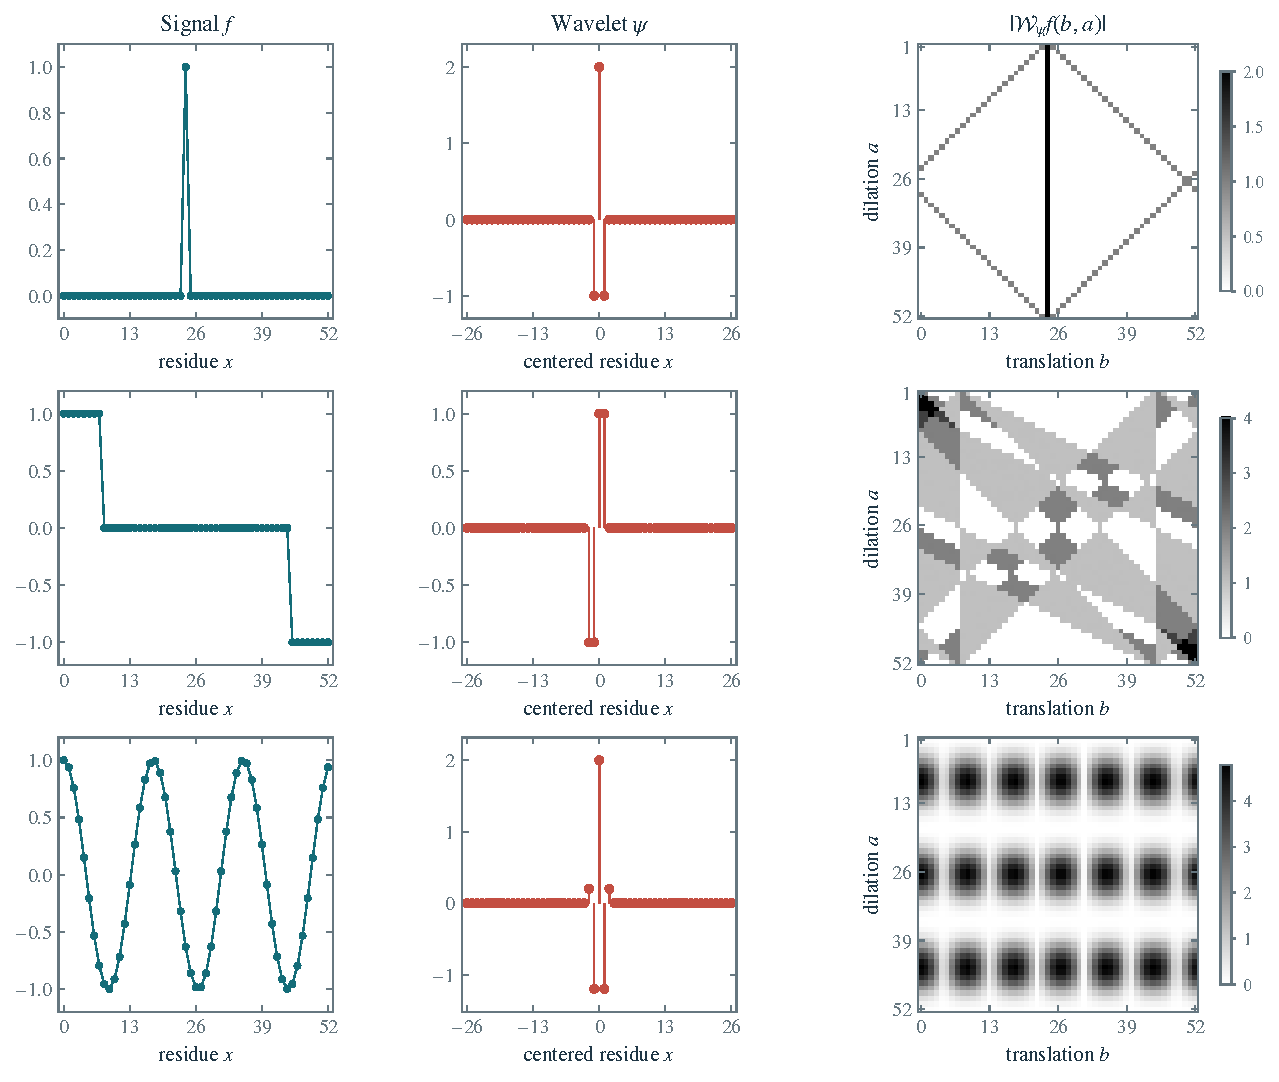
\includegraphics[width=\linewidth]{figures/chapter-linear-representations/finite-field-wavelets/figure.pdf}
\caption{Wavelets on $\FF_{53}$: the signal, the centered wavelet, and the magnitude of its affine-group transform. Translation $b$ is horizontal and nonzero dilation $a$ is vertical. Each row has its own indicated magnitude scale. The first signal has nonzero mean, which the mean-zero wavelet removes.}
\label{wavelets-finite-body}
\end{figure}
This finite-field construction is developed in \cite{flornes}. Its algebraic
dilations are permutations of residues, rather than a nested family of
Euclidean scales.
\end{exo}
